

\newlength{\colwidthA} \setlength{\colwidthA}{0.15\textwidth}
\newlength{\colwidthB} \setlength{\colwidthB}{0.2\textwidth}
\newlength{\colwidthC} \setlength{\colwidthC}{0.1\textwidth}
\newlength{\colwidthE} \setlength{\colwidthE}{0.10\textwidth}
\newlength{\colwidthF} \setlength{\colwidthF}{0.05\textwidth}
\newlength{\colwidthG} \setlength{\colwidthG}{0.15\textwidth}

{ \rowcolors{1}{ColorAlternatedRow}{}
\setlength\extrarowheight{4pt}
\begin{tabularx}{\linewidth}% tabularx implements a version of the tabular environment in which the widths of certain columns are calculated so that the table is a specified width
{%
  >{\setlength{\hsize}{.20\hsize}\raggedright\arraybackslash}X%
  >{\setlength{\hsize}{.25\hsize}\arraybackslash}X%
  >{\setlength{\hsize}{.15\hsize}\raggedright\arraybackslash}X%
  >{\setlength{\hsize}{.15\hsize}\raggedright\arraybackslash}X%
  >{\setlength{\hsize}{.10\hsize}\raggedright\arraybackslash}X%
  >{\setlength{\hsize}{.20\hsize}\raggedright\arraybackslash}X%
}
\hiderowcolors
    Product &
    Note &
    $f_C$, $\Delta f$ &
    Antennas &
    DK Price &
    Picture \\
\toprule
\endhead

\midrule
\multicolumn{6}{r}{Continued on next page} \\
\endfoot

\bottomrule
\endlastfoot
\showrowcolors

\href{https://www.omniradar.com/products/}{Omniradar RIC60A} &
High bandwidth. Presentation at SoC 2015\cite{Brouwer2015} &
60~GHz, 7~GHz &
On-chip, 1~Tx,~2~Rx &
\$4000 &
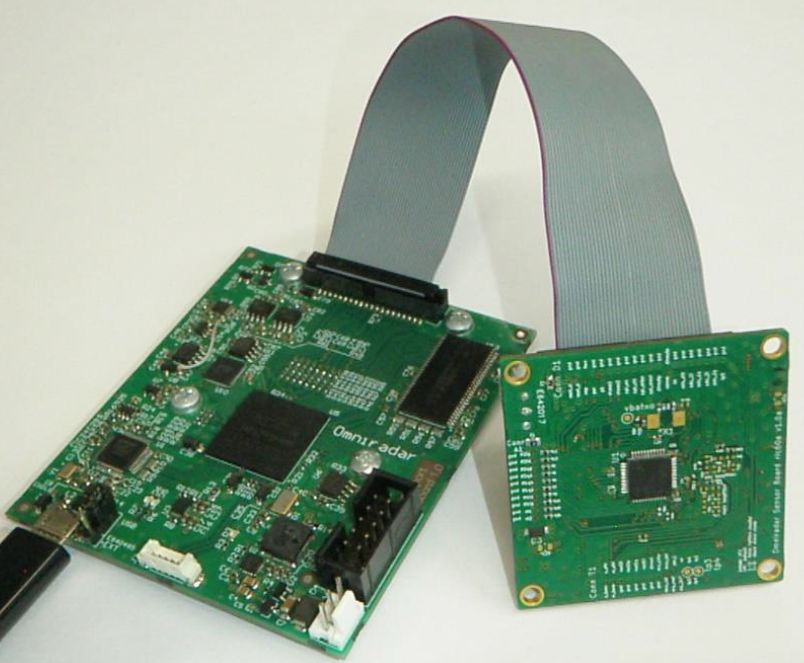
\includegraphics[width=\hsize,valign=t]{boards/img_omniradar.jpg}
\tabularnewline

\href{https://www.infineon.com/cms/en/product/promopages/soli/}{Google / Infineon Soli} &
Expected 2018. Sub-millimeter accuracy, running at over 10,000 frames per second \cite{Lien2016} &
60~GHz, 7~GHz &
In\nobreakdash-package, 2~Tx,~4~Rx &
? &
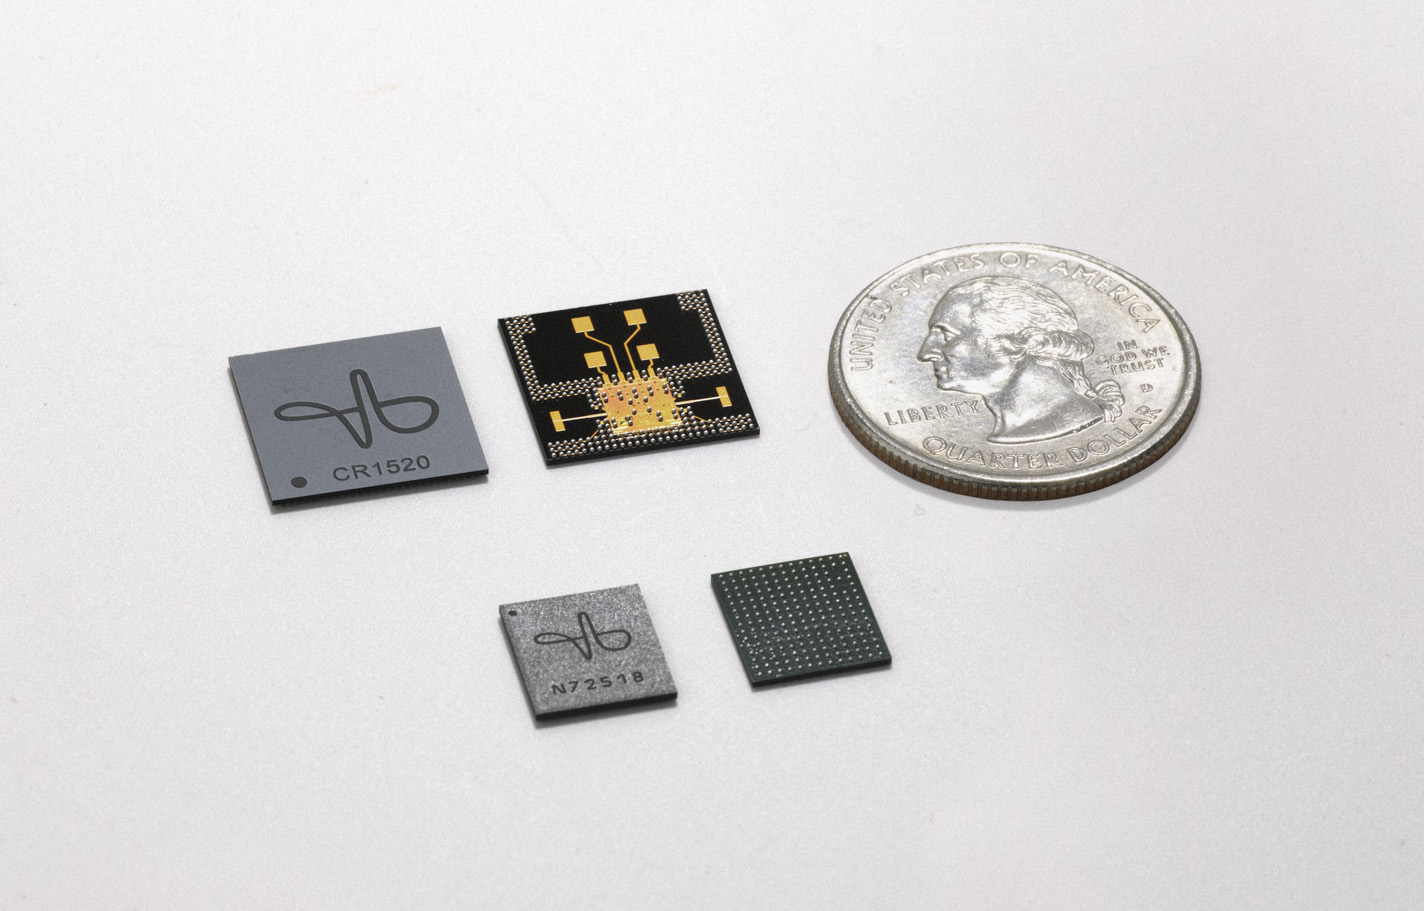
\includegraphics[width=\hsize,valign=t]{boards/img_soli.png}
\tabularnewline

\href{https://walabot.com/store/us/products/walabot-developer-pack.html}{Walabot Pro}&
3D configuration. Slow update rate&
6.8~GHz, 7~GHz &
On\nobreakdash-board, 9~Tx,~9~Rx&
\$599&
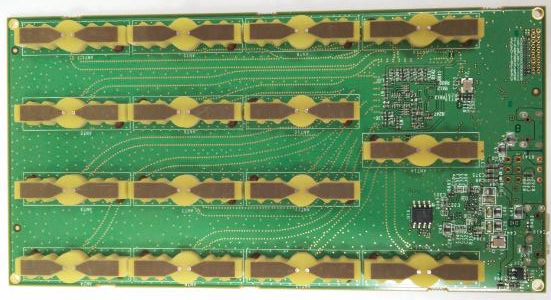
\includegraphics[width=\hsize,valign=t]{boards/img_walabot_1.png}
\tabularnewline

Bosch Prototype&
Prototype for In-wall pipe detection&
5.15~GHz, 6.7~GHz &
External, 2~Tx/Rx&
\$0&
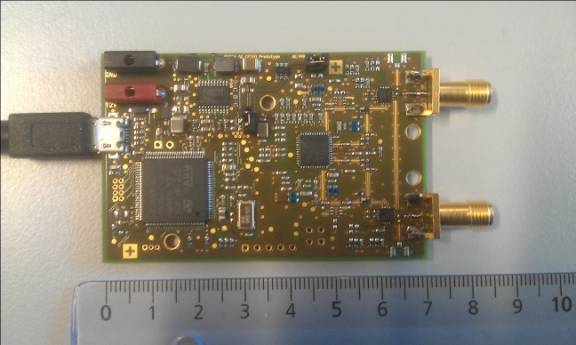
\includegraphics[width=\hsize,valign=t]{boards/img_bosch.jpg}
\tabularnewline

\href{http://www.siliconradar.de/evalkits_e.html}{Silicon Radar SiRad Simple}&
Has WiFi&
122~GHz, 6.4~GHz &
On-chip, 1~Tx,~1~Rx&
?&
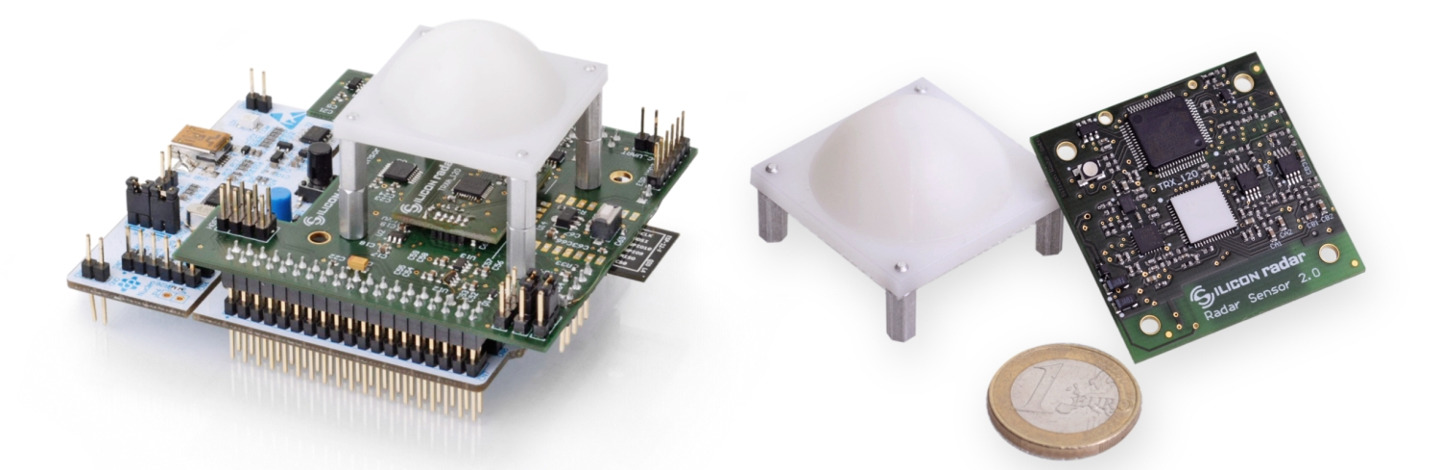
\includegraphics[width=\hsize,valign=t]{boards/img_silicon_radar.jpg}
\tabularnewline

\href{http://www.anokiwave.com/products/awmf-0117/index.html}{Anokiwave AWMF-0117}&
&
12.5~GHz, 4.5~GHz &
On-chip, 1~Tx/Rx&
?&
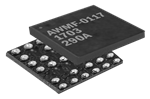
\includegraphics[width=\hsize,valign=t]{boards/img_anokiwave.png}
\tabularnewline

\href{Reuter2016}{NXP Cocoon Radar}&
Relatively small board. Presentation at FTF 2016\cite{Reuter2016}&
77~GHz, 4~GHz &
On\nobreakdash-board, 3~Tx,~4~Rx&
?&
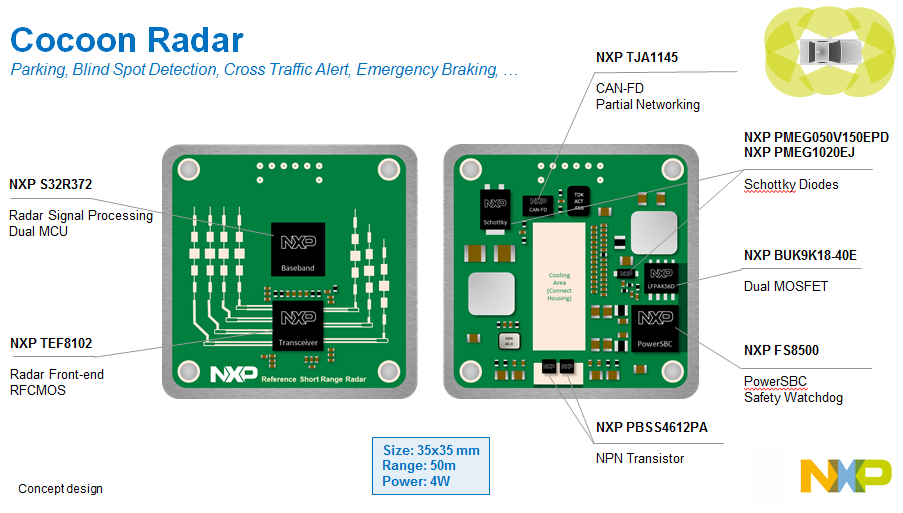
\includegraphics[width=\hsize,valign=t]{boards/img_cocoon.png}
\tabularnewline

\href{http://www.timedomain.com/products/pulson-440/}{TimeDomain P440}&
Can operate as multistatic radar or UWB communication node&
4~GHz, 1.7~GHz &
External, 2~Tx/Rx&
\$5000&
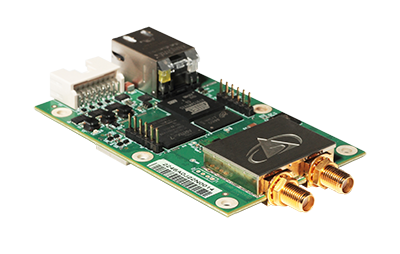
\includegraphics[width=\hsize,valign=t]{boards/img_p440.png}
\tabularnewline

\href{https://www.xethru.com/xethru-development-platform.html}{Novelda Xethru X4M03}&
&
8~GHz, 1.5~GHz &
On\nobreakdash-board, 1~Tx/Rx&
\$399&
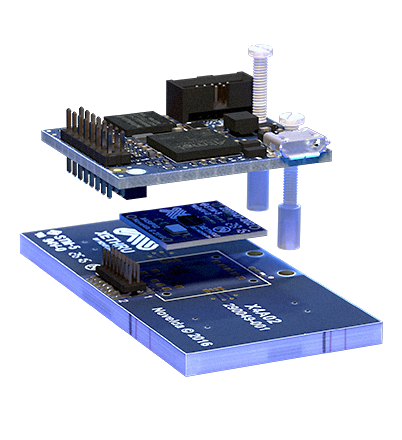
\includegraphics[width=\hsize,valign=t]{boards/img_xethru.png}
\tabularnewline

\href{https://www.rfbeam.ch/files/products/26/downloads/ProductBrief_MR2001_RD.pdf}{RFbeam MR2001\_RD}&
&
77~GHz, 1~GHz &
On\nobreakdash-board, 4~Tx,~6~Rx&
?&
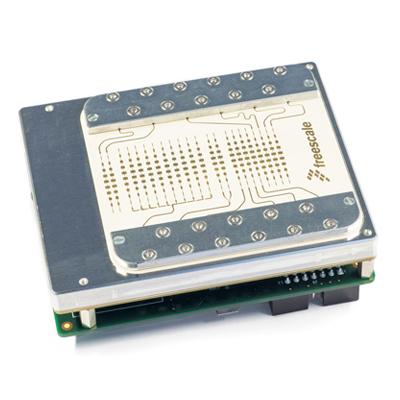
\includegraphics[width=\hsize,valign=t]{boards/img_rfbeam.jpg}
\tabularnewline

\href{http://www.inras.at/en/products/radarbook.html}{Inras 77Ghz Radarbook}&
Configurable FPGA processing chain&
77~GHz, 1~GHz &
On\nobreakdash-board, 4~Tx,~8~Rx&
\$7300&
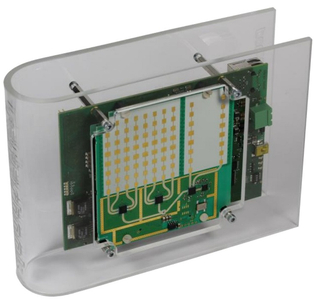
\includegraphics[width=\hsize,valign=t]{boards/img_radarbook.jpg}
\tabularnewline

\href{ http://www.acconeer.com/}{Acconeer A1}&
Sub-mm accuracy&
60~GHz, ? &
On-chip, ?&
?&
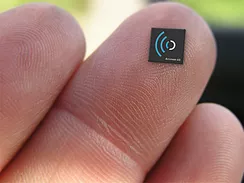
\includegraphics[width=\hsize,valign=t]{boards/img_acconeer.png}
\tabularnewline

\href{dkradarbook}{Inras 24Ghz Radarbook}&
&
24~GHz, 250~MHz &
On\nobreakdash-board, 4~Tx,~4~Rx&
\$7300&
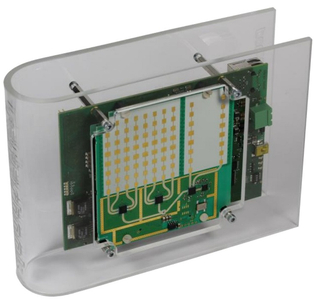
\includegraphics[width=\hsize,valign=t]{boards/img_radarbook.jpg}
\tabularnewline

\href{https://www.infineon.com/dgdl/Infineon-AN380_BGT24-RFB2412_user_manual-AN-v01_00-EN.pdf?fileId=5546d46259d9a4bf0159f9f1fa503f1d}{Infineon BGT24-RFB2412-EVAL}&
&
24~GHz, 250~MHz &
On\nobreakdash-board, 1~Tx,~2~Rx&
\$1333&
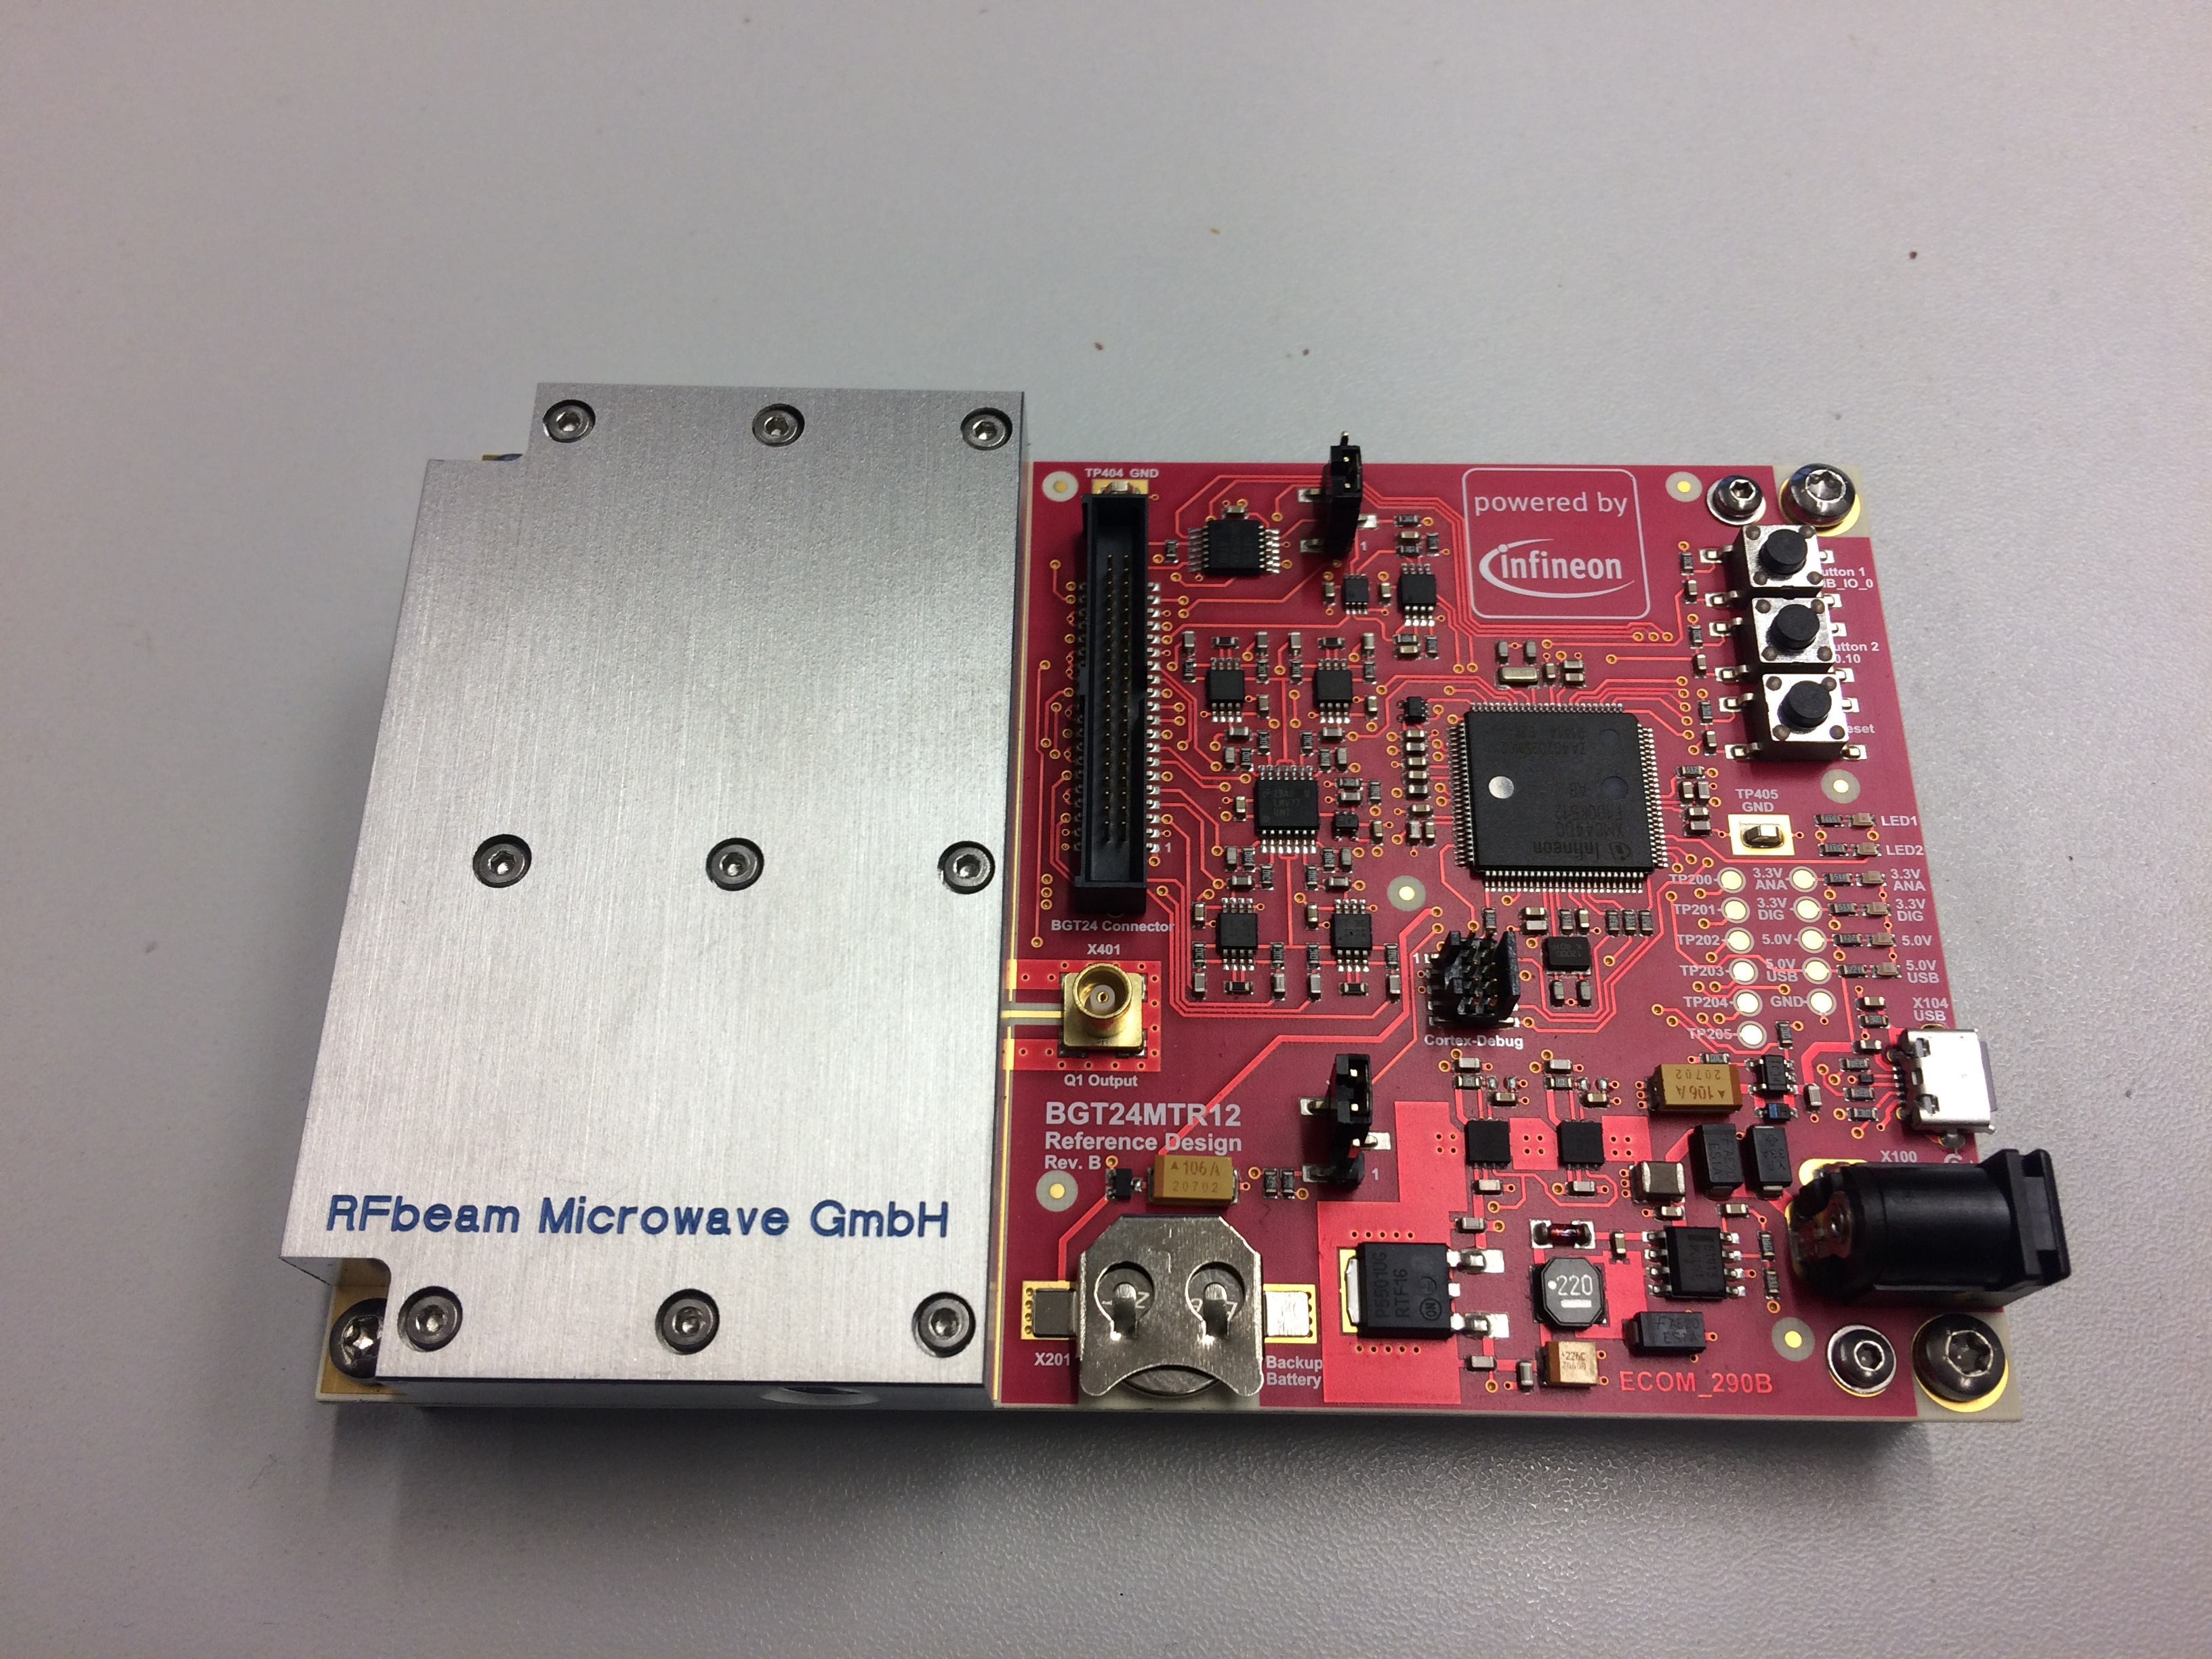
\includegraphics[width=\hsize,valign=t]{boards/img_bgt24.JPG}
\tabularnewline

\href{http://webshop.imst.de/dk-sr-1200e-development-platform-for-24-ghz-fmcw-radar-application.html
}{IMST DK-sR-1200e}&
&
24~GHz, 250~MHz &
On\nobreakdash-board, 1~Tx,~2~Rx&
\$3333&
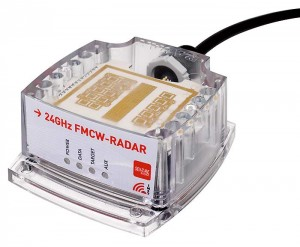
\includegraphics[width=\hsize,valign=t]{boards/img_IMST.jpg}
\tabularnewline

\href{http://www.innosent.de/fileadmin/media/dokumente/DATASHEETS_2016/Datenblatt_IVS-565.pdf}{InnoSenT IVS-565}&
&
24~GHz, 250~MHz &
On\nobreakdash-board, 1~Tx,~2~Rx&
?&
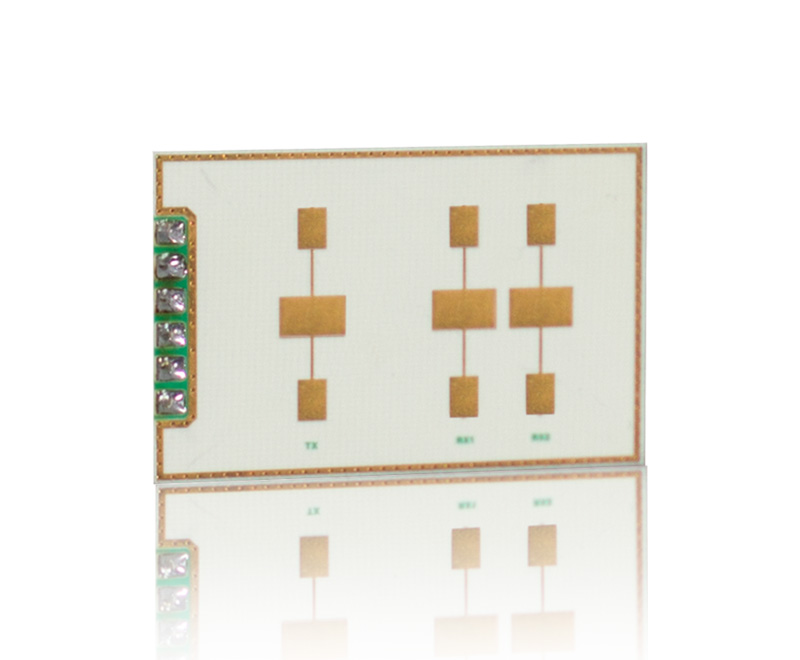
\includegraphics[width=\hsize,valign=t]{boards/img_innosent.jpg}
\tabularnewline

\href{http://www.st.com/content/st_com/en/products/evaluation-tools/product-evaluation-tools/automotive-ic-eval-boards/evb-strada431.html}{ST EVB-STradA431}&
SMA connectors for internal signals&
24~GHz, 250~MHz &
External, 1~Tx,~3~Rx&
?&
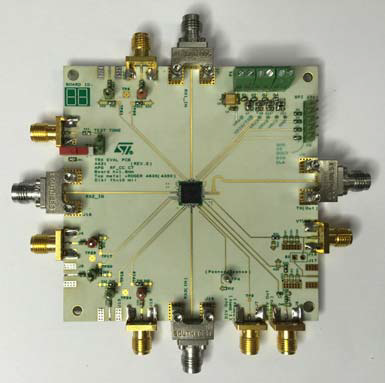
\includegraphics[width=\hsize,valign=t]{boards/img_ST.png}
\tabularnewline

\href{https://www.omnipresense.com/product/ops241-a/}{OmniPreSense OPS241-A}&
Arduino shield with BGT24LTR11&
24~GHz, 80~MHz &
On\nobreakdash-board, 1~Tx/Rx&
\$169&
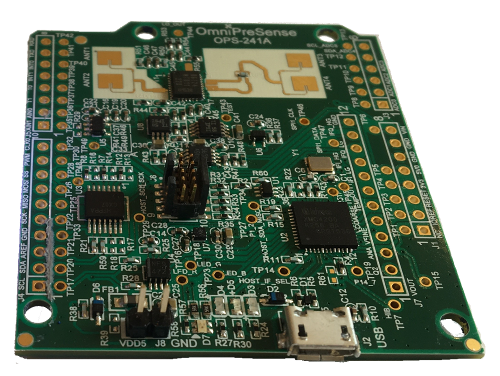
\includegraphics[width=\hsize,valign=t]{boards/img_omnipresense.png}
\tabularnewline


\bottomrule
\end{tabularx}

} % \rowcolors{1}{}{ColorAlternatedRow}


